%%%%%%%%%%%%%%%%%%%%%%%%%%%%%%%%%%%%%%%%%%%%%%%%%%%%%%%%%%%%%%%%%%%%%%%%%%%%%%%%
%% 
\cleardoubleoddpage%  Make sure to start each chapter on a new odd page
\chapter{Experiments and Results}
\section{Experimental Setup}
We conducted our experiments on a machine equipped with an AMD Ryzen 5 1600 CPU and a NVIDIA GeForce GTX 1070 GPU. The initial step involved establishing a baseline performance to later asses both models under various conditions. We utilized the PyTorch framework~\cite{paszke2019pytorch} for training, taking advantage of its pre-built functions for neural network training. The Adam optimizer was employed throughout the training processes, along with the \lstinline{ReduceLROnPlateau} learning rate scheduler set to a patience of 5 epochs. Additionally, we implemented early stopping, evaluating the model's performance on the validation set after each training epoch, with a patience threshold of 10 epochs.\\
For optimal baseline determination, we used the Optuna framework~\cite{akiba2019optuna} for hyperparameter optimization. The objectives included maximizing the AUC-Score and Balanced Accuracy on the validation set while minimizing the epochs required to achieve respectable results. This process yielded the following hyperparameters for our models:\\\\
\textbf{VAE}: The optimal batch size was determined to be 32, with a learning rate of 1e-4. The \textit{nf} hyperparameter in the DCGAN architecture, which affects the depth of feature maps in both the generator and discriminator, was found to be most effective at 128. The size of the latent space vector was set to 128, and the alpha weighting factor balancing the Mean Squared Error loss and the Kullback-Leibler Divergence was adjusted to 0.5.\\\\
\textbf{GMADE}: A batch size of 128 and a learning rate of 1e-3 were optimal for this model. Using a single mask configuration without resampling the mask during training, we achieved the best results with a hidden layer structure of [256, 156, 512].
\section{Generalization Capabilities}
The ability of a machine learning model to generalize to unseen data is as crucial as its performance during training. We evaluated the generalization of our models using the test set, as described in \autoref{method:data-splitting}, with an 80/20 split. We assessed all three input orderings and their mean ensemble for the GMADE model.\\
We established a binary classification threshold based on anomaly scores to gauge the Balanced Accuracy, True Positive Rate (TPR), and True Negative Rate (TNR). This threshold was determined using the validation set, which includes some anomalous data. We tested each anomaly score as a potential threshold, selecting the one that maximized Balanced Accuracy on the validation set. This approach underpins the weakly-supervised aspect of our methodology.

\begin{table}[h!]
    \centering
    \caption{Experiment Results for VAE and GMADE Models with Different Orderings}
    \begin{tabular}{|l|l|c|c|}
    \hline
    \textbf{Model} & \textbf{Metric} & \textbf{Validation Set} & \textbf{Test Set} \\
    \hline
    \multirow{4}{*}{VAE} 
    & ROC-AUC & \textbf{0.64} & \textbf{0.62} \\
    & BALACC  & \textbf{0.61} & \textbf{0.61} \\
    & TPR     & 0.84 & 0.84 \\
    & TNR     & 0.39 & 0.39 \\
    \hline
    \multirow{4}{*}{GMADE (Forward)}
    & ROC-AUC & 0.59 & 0.57 \\
    & BALACC  & 0.57 & 0.57 \\
    & TPR     & \textbf{0.90} & \textbf{0.90} \\
    & TNR     & 0.24 & 0.24 \\
    \hline
    \multirow{4}{*}{GMADE (Backward)}
    & ROC-AUC & 0.58 & 0.57 \\
    & BALACC  & 0.57 & 0.57 \\
    & TPR     & 0.78 & 0.78 \\
    & TNR     & 0.36 & 0.37 \\
    \hline
    \multirow{4}{*}{GMADE (Mid-Frame)}
    & ROC-AUC & 0.56 & 0.55 \\
    & BALACC  & 0.56 & 0.57 \\
    & TPR     & 0.86 & 0.86 \\
    & TNR     & 0.27 & 0.29 \\
    \hline
    \multirow{4}{*}{GMADE (Ensemble)}
    & ROC-AUC & 0.59 & 0.58 \\
    & BALACC  & 0.57 & 0.56 \\
    & TPR     & 0.71 & 0.70 \\
    & TNR     & \textbf{0.42} & \textbf{0.43} \\
    \hline
    \end{tabular}
\end{table}

Our performance results indicate that with its reconstruction-based approach, the Variational Autoencoder (VAE) slightly outperforms the GMADE models in accuracy and AUC-Score. However, all models show a notable number of false positives, possibly due to the high environmental noise in the recordings the models assume to be anomalies. The ensemble GMADE model demonstrated the highest TNR, indicating a better balance in minimizing false positives while identifying healthy patients. Interestingly, while the ensemble improved the TNR and the AUC-Score marginally, it did not enhance the Balanced Accuracy compared to individual orderings due to the lower TPR.\\
All models are competitive to the weakly-supervised approach introduced by~\cite{cozzatti2022variational} and allow for a more nuanced inspection of the capabilities of the models.
\section{Age and Gender Differences in Model Accuracy}
Machine learning algorithms often suffer from imbalances in gender representation, mainly due to insufficient data from females, youths, and older individuals. This imbalance is critical in medical applications where fairness across different genders and age groups must be assured. To address this, we evaluated our models' performance on various subgroups within our dataset, using thresholds established as previously described.\\
\textbf{Gender}: We analyzed the models' performance by filtering the test set for male and female samples separately.

\begin{table}[h!]
    \centering
    \caption{Experiment Results by Gender for VAE and GMADE Models}
    \begin{tabular}{|l||c|c||c|c||c|c||c|c|}
    \hline
    \textbf{Model} & \multicolumn{2}{c||}{\textbf{ROC-AUC}} & \multicolumn{2}{c||}{\textbf{BALACC}} & \multicolumn{2}{c||}{\textbf{TPR}} & \multicolumn{2}{c|}{\textbf{TNR}} \\
    \cline{2-9}
    & \textbf{F} & \textbf{M} & \textbf{F} & \textbf{M} & \textbf{F} & \textbf{M} & \textbf{F} & \textbf{M} \\
    \hline
    VAE & \textbf{0.59} & \textbf{0.64} & \textbf{0.59} & \textbf{0.61} & 0.81 & 0.84 & 0.37 & 0.39 \\
    GMADE (Forward) & 0.55 & 0.58 & 0.58 & 0.56 & \textbf{0.92} & \textbf{0.89} & 0.25 & 0.23 \\
    GMADE (Backward) & 0.54 & 0.58 & 0.54 & 0.6 & 0.75 & 0.80 & 0.33 & 0.39 \\
    GMADE (Mid-Frame) & 0.52 & 0.57 & 0.56 & 0.58 & 0.84 & 0.87 & 0.27 & 0.29 \\
    GMADE (Ensemble) & 0.56 & 0.59 & 0.56 & 0.56 & 0.68 & 0.7 & \textbf{0.44} & \textbf{0.42} \\
    \hline
    \end{tabular}
\end{table}
All models, except the ensemble GMADE, display reduced accuracy for female recordings. Interestingly, the ensemble GMADE maintains equal Balanced Accuracy across genders, although it exhibits a slightly lower AUC-Score for females. Among all models, the VAE consistently performs better in both male and female subsets. However, the difference in its accuracy between genders is more pronounced than in the ensemble GMADE. Despite achieving a high True Positive Rate, the forward-ordered GMADE tends to generate many false positives. In contrast, the Ensemble achieves the highest True Negative Rate (TNR).\\
This observed discrepancy in gender-based accuracy is likely due to an imbalance in the dataset composition. Of the 6.898 recorded breathing cycles, 4.485 originate from male patients, while only 2.413 are from female patients, suggesting a potential bias in data representation.\\\\
\textbf{Age}: We categorized recordings into three age groups: (0-7], (7-70], and (70-85]. These groups were chosen for their comparative size and representativeness, with the youngest patient being less than a year old and the oldest at 85.

\begin{table}[h!]
    \centering
    \caption{Performance by Age Group for VAE and GMADE Models}
    \begin{tabular}{|l|l|c|c|c|c|}
    \hline
    \textbf{Age Group} & \textbf{Model} & \textbf{ROC-AUC} & \textbf{BALACC} & \textbf{TPR} & \textbf{TNR} \\
    \hline
    \multirow{5}{*}{(0-7]} 
    & VAE & 0.49 & 0.52 & 0.25 & \textbf(0.8) \\
    & GMADE (Forward) & 0.50 & 0.47 & \textbf(0.48) & 0.47 \\
    & GMADE (Backward) & 0.52 & 0.53 & 0.33 & 0.73 \\
    & GMADE (Mid-Frame) & 0.52 & 0.51 & 0.46 & 0.56 \\
    & GMADE (Ensemble) & \textbf(0.62) & \textbf(0.56) & 0.36 & 0.76 \\
    \hline
    \multirow{5}{*}{(7-70]} 
    & VAE & \textbf(0.6) & \textbf(0.58) & 0.85 & 0.30 \\
    & GMADE (Forward) & 0.56 & 0.54 & \textbf(0.90) & 0.18 \\
    & GMADE (Backward) & 0.55 & 0.56 & 0.83 & 0.30 \\
    & GMADE (Mid-Frame) & 0.54 & 0.55 & 0.83 & 0.30 \\
    & GMADE (Ensemble) & 0.56 & 0.54 & 0.69 & \textbf(0.39) \\
    \hline
    \multirow{5}{*}{(70-85]} 
    & VAE & \textbf(0.6) & \textbf(0.59) & 0.83 & 0.34 \\
    & GMADE (Forward) & 0.56 & 0.54 & \textbf(0.9) & 0.18 \\
    & GMADE (Backward) & 0.55 & 0.56 & 0.83 & 0.30 \\
    & GMADE (Mid-Frame) & 0.54 & 0.55 & 0.87 & 0.22 \\
    & GMADE (Ensemble) & 0.52 & 0.54 & 0.73 & \textbf(0.35) \\
    \hline
    \end{tabular}
\end{table}

A distinct pattern emerges: almost all models struggle with recordings from the (0-7] age group. Unlike older age groups, where anomalies are detected more reliably but with higher false positives, younger patients' anomalies are often missed, while normal conditions are identified more accurately. The exception is the ensemble GMADE, which is still able to achieve a respectable accuracy in the youngest group, outperforming all individual orderings and VAE. In the older groups, VAE is performing better than GMADE.\\
The difficulty in analyzing younger patients' data could stem from their faster breathing cycles compared to older subjects. The average cycle length for patients older than seven is 2.37 seconds, while for those seven or younger, it is 1.64 seconds, potentially making anomalous sounds too short for effective detection.

\section{Model Sensitivity to Noise}
A critical measure of a model's practical applicability is its tolerance to noise. We assessed the resilience of our models against varying noise levels. Noise was generated by sampling from a normal distribution and added to the test set's signal at different Signal to Noise Ratios (SNRs) using PyTorch's \lstinline{torchaudio.functional.add_noise}. SNR, measured in decibels, compares the background noise level to the original signal strength. A lower SNR indicates stronger noise: positive SNR values imply the signal is stronger than the noise, negative values indicate the noise is stronger, and 0 dB SNR signifies equal loudness for both noise and signal.\\
Our investigation began with an SNR of 30 dB, where the original signal was dominant, and progressively increased the noise level to 20 dB, 10 dB, and finally 0 dB. We then plotted the Balanced Accuracy of our models against these SNR values.
\begin{figure}[h!]
    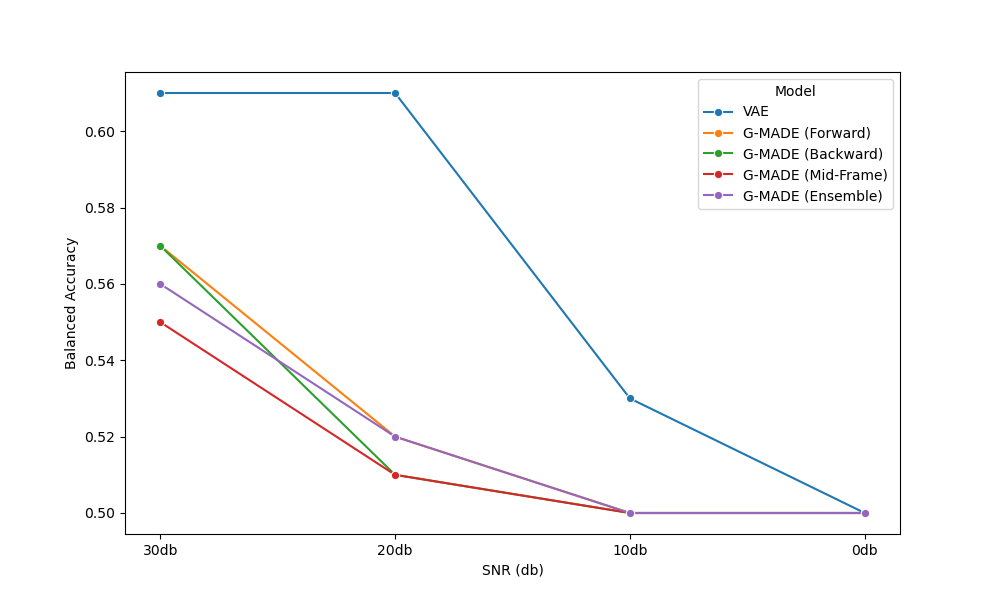
\includegraphics[width=\linewidth]{images/snr_balacc}
    \caption{
    Balanced Accuracy vs SNR Noise Level for Different Models
}
\end{figure}

As anticipated, the Balanced Accuracy of all models decreases with increasing noise. While we observed near-original performance at 30 dB SNR, a significant drop is noticeable at 20dB for all GMADE models. Interestingly, the VAE could keep the same accuracy at 20dB SNR compared to 30dB SNR and performs best at these levels of noise. However, all models fail to have meaningful separation power from 10dB SNR.\\
It is noteworthy that the original signal already contained substantial environmental noise. Nevertheless, the VAE seems to be more robust against noise in the sound signal.
\section{Model Performance on Crackles and Wheezes}
The ability to distinguish between crackles and wheezes is vital in diagnosing different respiratory conditions, given their distinct acoustic characteristics. To assess this, we modified the test set to evaluate performance with crackles and wheezes separately, alongside healthy sounds.

\begin{table}[h!]
    \centering
    \caption{Model Performance for Crackles and Wheezes}
    \begin{tabular}{|l|c|c|c|c||c|c|c|c|}
    \hline
    & \multicolumn{4}{c||}{\textbf{Crackles}} & \multicolumn{4}{c|}{\textbf{Wheezes}} \\
    \cline{2-9}
    \textbf{Model} & \textbf{ROC-AUC} & \textbf{BALACC} & \textbf{TPR} & \textbf{TNR} & \textbf{ROC-AUC} & \textbf{BALACC} & \textbf{TPR} & \textbf{TNR} \\
    \hline
    VAE & \textbf{0.60} & \textbf{0.60} & 0.81 & 0.38 & \textbf{0.64} & \textbf{0.61} & 0.84 & 0.37 \\
    GMADE (Forward) & 0.55 & 0.57 & \textbf{0.91} & 0.24 & 0.57 & 0.55 & 0.87 & 0.23 \\
    GMADE (Backward) & 0.55 & 0.56 & 0.75 & 0.36 & 0.59 & 0.59 & 0.82 & 0.37 \\
    GMADE (Mid-Frame) & 0.53 & 0.56 & 0.84 & 0.29 & 0.58 & 0.57 & \textbf{0.86} & 0.29 \\
    GMADE (Ensemble) & 0.57 & 0.56 & 0.7 & \textbf{0.43} & 0.57 & 0.55 & 0.67 & \textbf{0.43} \\
    \hline
    \end{tabular}
\end{table}

The results do not indicate a clear trend between the performance for wheezes and crackles. While the AUC-Scores for wheezes is higher than those for crackles, the Balanced Accuracy does not confirm this tendency. Among the GMADE models, backward ordering performs most effectively on wheezes, whereas forward ordering is most effective on crackles. Notably, the VAE model consistently achieves the highest accuracy for wheezes and crackles. Interestingly, as seen in previous tests, the ensemble GMADE exhibits the highest True Negative Rate (TNR) for both crackles and wheezes.\\
Considering the dataset distribution of 1.864 crackles to 886 wheezes, it is intriguing that the models perform similar across crackles and wheezes despite their substantially lower representation. It shows that the models are able to detect both respiratory phenomena.

\section{Impact of Hyperparameter Variations}
Optimizing hyperparameters is a crucial yet challenging task in machine learning model training. We utilized the Optuna optimization framework for our models, conducting 30 studies for each model to analyze the relative importance of various hyperparameters in achieving high Balanced Accuracy. A higher value indicates greater importance, suggesting that a modification in that hyperparameter would significantly impact the results.

\begin{figure}[h!]
    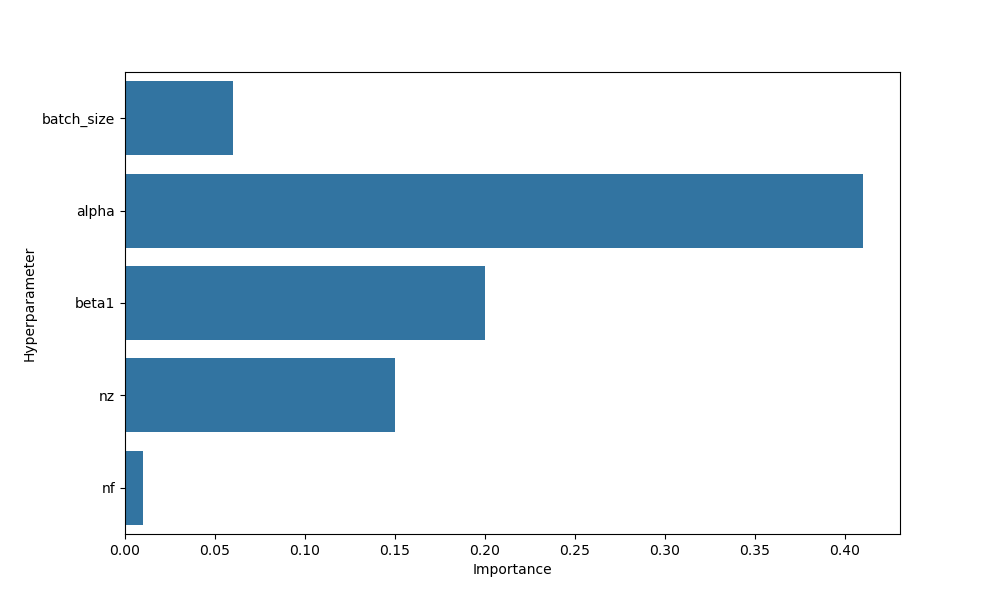
\includegraphics[width=\linewidth]{images/importances_vae}
    \caption{
    Hyperparameter performance in VAE training
}
\end{figure}

In the case of the Variational Autoencoder (VAE), the most influential factor is the \lstinline{alpha} weighting term, which balances the Mean Square Error and Kullback-Leibler Divergence in the overall loss function. The \lstinline{beta1} parameter of the Adam optimizer and the dimension of the latent vector (\lstinline{nz}) also play significant roles. Interestingly, the \lstinline{nf} parameter, which affects the feature depth in the DCGAN Generator and Discriminator, has a minimal impact on overall model performance.

\begin{figure}[h!]
    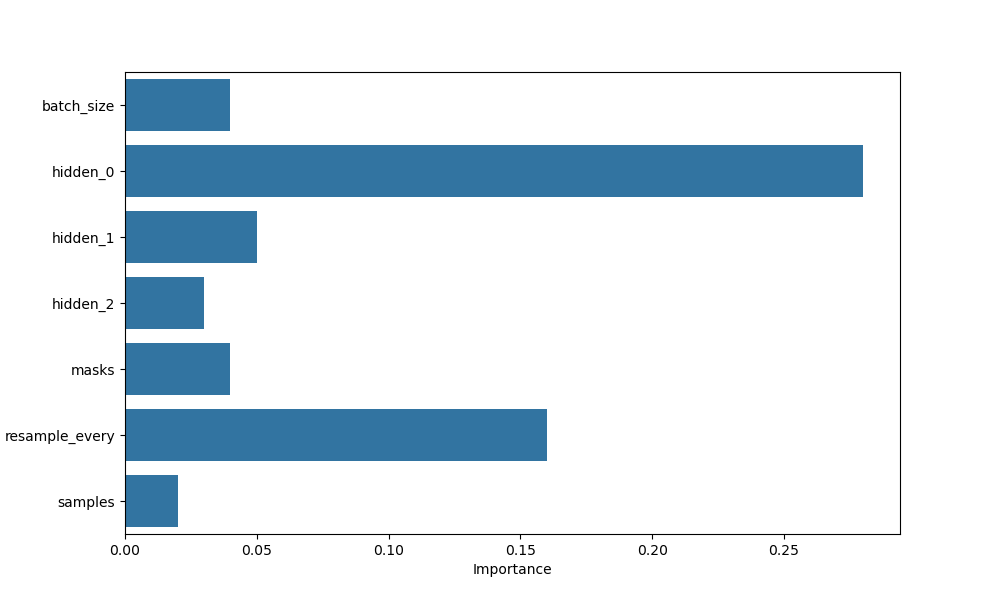
\includegraphics[width=\linewidth]{images/importances_gmade}
    \caption{
    Hyperparameter performance in GMADE (forward) training
}
\end{figure}

The GMADE model, featuring hyperparameters for its hidden layers, inherently requires more tuning than the VAE. The size of the first hidden layer is paramount in training GMADE, followed by the frequency of mask resampling during forward passes. The subsequent hidden layers, the number of different weight masks, and the frequency of mask resampling per forward pass all show similar and relatively low importance.

\section{Assessment of Data Splitting at Recording Level}
In line with concerns mentioned in \autoref{method:data-splitting}, splitting data at the breathing cycle level risks overestimating the model generalization capabilities, as cycles from the same patient might appear in training and test sets. To address this, we examined the impact of our custom-designed recording level split on model performance.

\begin{figure}[h!]
    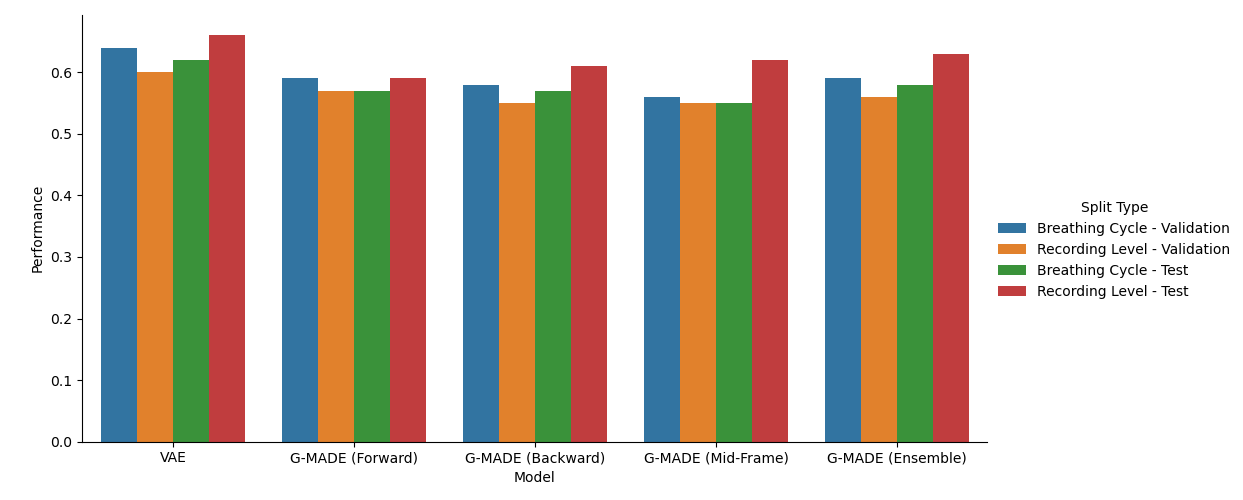
\includegraphics[width=\linewidth]{images/split_performance}
    \caption{
    Model performance on different data split
}
\end{figure}

The results demonstrate effective generalization across models for both data splits. However, an interesting trend can be observed: while the test set performance was marginally lower than the validation set for the breathing cycle level split, it improved for the recording level split. This improvement in the test set performance for the recording level split might be attributed to a fortunate data division, indicating that the split could be unintentionally biased or more representative of the model's capabilities.

\section{Comparison of Feature Extraction Methods: MFCC vs. MelSpectrogram}
MFCCs and MelSpectrograms are widespread for representing sound data in machine learning but offer different advantages. MelSpectrograms are known for better human interpretability and retaining more temporal information compared to MFCCs. To evaluate the impact of these differences, we adapted our preprocessing as described in \autoref{method:preprocessing}, replacing \lstinline{torchaudio.transforms.MFCC} with \lstinline{torchaudio.transforms.MelSpectrogram} and retrained all models with the new feature representation.

\begin{table}[h!]
    \centering
    \caption{Experiment Results for VAE and GMADE Models using MelSpectrograms}
    \begin{tabular}{|l|l|c|c|c|}
    \hline
    \textbf{Model} & \textbf{Metric} & \textbf{Validation Set} & \textbf{Test Set} & \textbf{Test Set (Dropout)} \\
    \hline
    \multirow{4}{*}{VAE} 
    & ROC-AUC & 0.46 & 0.44 & - \\
    & BALACC  & 0.51 & 0.5 & - \\
    & TPR     & 0.98 & 0.96 & - \\
    & TNR     & 0.04 & 0.04 & - \\
    \hline
    \multirow{4}{*}{GMADE (Forward)}
    & ROC-AUC & \textbf{0.57} & \textbf{0.54} & \textbf{0.55} \\
    & BALACC  & \textbf{0.56} & \textbf{0.53} & 0.56 \\
    & TPR     & 0.36 & 0.34 & 0.88 \\
    & TNR     & 0.77 & 0.71 & 0.24 \\
    \hline
    \multirow{4}{*}{GMADE (Backward)}
    & ROC-AUC & 0.39 & 0.39 & 0.4 \\
    & BALACC  & 0.50 & 0.50 & 0.5 \\
    & TPR     & 1.0 & 1.0 & 1.0 \\
    & TNR     & 0.0 & 0.0 & 0.0 \\
    \hline
    \multirow{4}{*}{GMADE (Mid-Frame)}
    & ROC-AUC & 0.49 & 0.44 & 0.54 \\
    & BALACC  & 0.54 & 0.51 & 0.56 \\
    & TPR     & 0.28 & 0.28 & 0.92 \\
    & TNR     & 0.80 & 0.75 & 0.20 \\
    \hline
    \multirow{4}{*}{GMADE (Ensemble)}
    & ROC-AUC & 0.5 & 0.46 & 0.53 \\
    & BALACC  & 0.54 & 0.50 & \textbf{0.57} \\
    & TPR     & 0.41 & 0.37 & 0.91 \\
    & TNR     & 0.68 & 0.63 & 0.22 \\
    \hline
    \end{tabular}
\end{table}

Our findings reveal a significant variance in model performance when using MelSpectrograms compared to MFCCs. The Variational Autoencoder (VAE) could not learn any representation of normal data points, as indicated by the accuracy close to random behavior. The forward GMADE model maintains performance close to its MFCC counterpart but shows reduced generalization to the test set. The backward, mid-frame, and ensemble GMADE models suffer notable performance declines, especially in test set generalization.\\
Incorporating dropout (with $p=0.3$) in the Masked Autoencoder models improved their generalization capabilities. Notably, the forward, ensemble and mid-frame GMADE models approached performances similar to those achieved with MFCCs. However, the backward ordering model failed to benefit from dropout and could not learn any meaningful pattern.\\
These results suggest that GMADE models possess a degree of flexibility regarding input features, effectively accommodating both MelSpectrograms and MFCCs. However, our implementation of the Variational Autoencoder did not perform as well with MelSpectrograms. This could imply that the VAE architecture is struggling with the level of detail in the MelSpectrogram representation and can not retrieve the characteristics that make up a normal breathing cycle and may be more suited to the feature representation provided by MFCCs due to their compact and efficient encapsulation of relevant sound characteristics. Further refinements in the VAE's architecture or its training process might be needed to handle better the richer temporal information presented by MelSpectrograms.

\section{Comparative Analysis and Discussion}
We now want to provide a comprehensive analysis and discussion of the experiments' findings to determine how well reconstruction-based and density-estimation-based methods are suited for anomaly detection in respiratory sounds.
The Variational Autoencoder (VAE), our reconstruction-based model, showed significant effectiveness in our experiments. Its primary strength lies in its ability to learn a compact representation of normal breathing cycles, facilitating effective anomaly detection through reconstruction error measurement. Across various datasets, including different noise levels, age groups, and genders, the VAE consistently outperformed with higher AUC-Score and Balanced Accuracy.\\
Despite these strengths, the VAE's performance was less effective with MelSpectrograms, indicating a possible limitation in processing rich temporal information. Additionally, the VAE demonstrated greater variance in accuracy between genders and age groups, suggesting a potential sensitivity to data imbalances.\\
GMADE, employing density estimation, showcased its adaptability with different feature representations, maintaining relatively stable performance with both MFCCs and MelSpectrograms. Its ensemble approach notably enhanced the True Negative Rate, underlining its efficacy in minimizing false positives. However, GMADE generally scored lower in AUC-Score and Balanced Accuracy than VAE, except in the analysis of infant and child respiratory sounds, where it performed comparably well. This observation and its compatibility with MelSpectrogram features suggest GMADE's potential to handle nuanced temporal information. The ensemble strategy significantly contributes to the model's performance and stability.\\

\begin{table}[h!]
    \centering
    \caption{Comparison of Proposed Models with Existing Literature\\(80/20 Split, Test Set)}
    \begin{tabular}{|l|c|c|c|c|}
    \hline
    \textbf{Model} & \textbf{ROC-AUC} & \textbf{BALACC} & \textbf{TPR} & \textbf{TNR} \\
    \hline
    VAE (Ours) & \textbf{0.62} & \textbf{0.61} & \textbf{0.84} & 0.39 \\
    VAE (Cozzatti et al.)~\cite{cozzatti2022variational} & 0.61 & 0.60 & 0.58 & \textbf{0.61} \\
    GMADE (Ensemble) & 0.58 & 0.56 & 0.7 & 0.43 \\
    \hline
    \end{tabular}
\end{table}


Reconstruction-based (VAE) and density-estimation-based (GMADE) show promising respiratory sound anomaly detection capabilities and enable weakly-supervised learning in this domain. However, VAE's superior accuracy, noise robustness, and overall generalization capabilities make it a more suitable choice for this specific application. However, the decision on the model selection should also account for task-specific requirements, such as dataset characteristics and the importance of reducing false positives. 
%% 
%%%%%%%%%%%%%%%%%%%%%%%%%%%%%%%%%%%%%%%%%%%%%%%%%%%%%%%%%%%%%%%%%%%%%%%%%%%%%%%%
